\documentclass[tikz,border=8pt]{standalone}

\usepackage[T1]{fontenc}
\usepackage{lmodern}
\usetikzlibrary{arrows.meta,backgrounds,calc,positioning}

\definecolor{flowblue}{HTML}{0072B2}
\definecolor{flowgreen}{HTML}{009E73}
\definecolor{flowbrown}{HTML}{8C564B}
\definecolor{flowpurple}{HTML}{6F4EA1}
\definecolor{floworange}{HTML}{D55E00}
\definecolor{ink}{HTML}{243447}
\definecolor{mutedink}{HTML}{52606D}
\definecolor{linegray}{HTML}{9AA5B1}
\definecolor{panel}{HTML}{F5F7FA}
\definecolor{ownedfill}{HTML}{E8F1F8}
\definecolor{storefill}{HTML}{FFF1CC}
\definecolor{externalfill}{HTML}{F3ECF8}

\tikzset{
  box/.style={
    draw=linegray,
    fill=white,
    rounded corners=2pt,
    line width=0.6pt,
    minimum height=10mm,
    text width=30mm,
    align=center,
    font=\sffamily\small,
    text=ink,
    inner sep=4pt
  },
  actor/.style={box,text width=24mm},
  component/.style={box,fill=ownedfill},
  store/.style={box,fill=storefill,text width=24mm},
  external/.style={box,fill=externalfill,text width=34mm},
  network/.style={box,text width=26mm},
  boundary title/.style={font=\sffamily\bfseries\large,text=ink,anchor=west},
  flow/.style={-{Latex[length=3mm,width=2.2mm]},line width=1.6pt},
  story one/.style={flow,draw=flowblue},
  story two/.style={flow,draw=flowgreen},
  story three/.style={flow,draw=flowbrown},
  story four/.style={flow,draw=flowpurple},
  story five/.style={flow,draw=floworange},
  relation/.style={draw=linegray,line width=1.1pt},
  edge label/.style={
    fill=none,
    inner xsep=1.5pt,
    inner ysep=3pt,
    font=\sffamily\scriptsize,
    text=mutedink,
    align=center
  },
  every node/.append style={font=\sffamily}
}

\newcommand{\storyStep}[2]{%
  \tikz[baseline=(step.base)]
    \node[circle,fill=#1,text=white,inner sep=1.1pt,
      font=\sffamily\bfseries\tiny] (step) {#2};%
}

\begin{document}
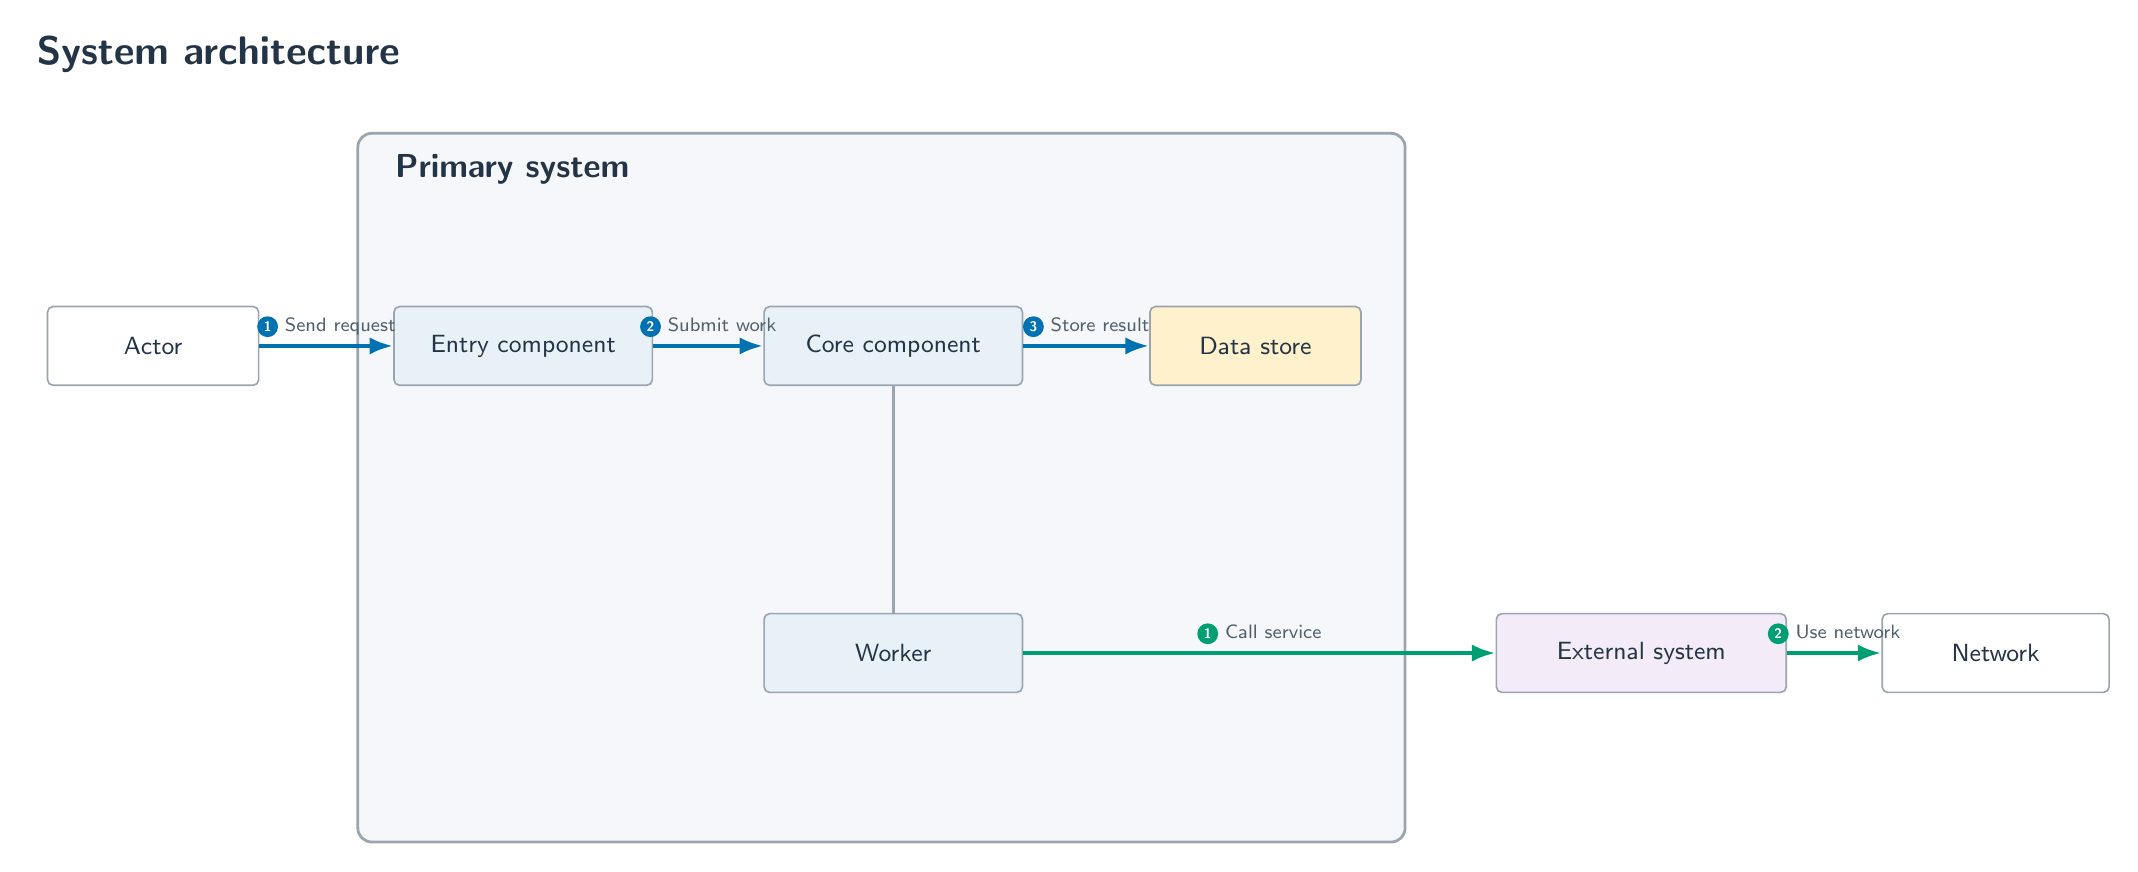
\begin{tikzpicture}[x=1cm,y=1cm]
  \node[font=\sffamily\bfseries\Large,text=ink,anchor=west]
    at (0,11.2) {System architecture};

  \begin{scope}[on background layer]
    \fill[panel,rounded corners=5pt] (4.2,1.2) rectangle (17.5,10.2);
    \draw[linegray,rounded corners=5pt,line width=1pt]
      (4.2,1.2) rectangle (17.5,10.2);
  \end{scope}

  \node[boundary title] at (4.55,9.75) {Primary system};

  \node[actor] (actor) at (1.6,7.5) {Actor};
  \node[component] (entry) at (6.3,7.5) {Entry component};
  \node[component] (service) at (11.0,7.5) {Core component};
  \node[store] (store) at (15.6,7.5) {Data store};
  \node[component] (worker) at (11.0,3.6) {Worker};
  \node[external] (external) at (20.5,3.6) {External system};
  \node[network] (network) at (25.0,3.6) {Network};

  \draw[story one] (actor.east) --
    node[edge label,above] {\storyStep{flowblue}{1} Send request}
    (entry.west);
  \draw[story one] (entry.east) --
    node[edge label,above] {\storyStep{flowblue}{2} Submit work}
    (service.west);
  \draw[story one] (service.east) --
    node[edge label,above] {\storyStep{flowblue}{3} Store result}
    (store.west);
  \draw[relation] (service.south) -- (worker.north);
  \draw[story two] (worker.east) --
    node[edge label,above] {\storyStep{flowgreen}{1} Call service}
    (external.west);
  \draw[story two] (external.east) --
    node[edge label,above] {\storyStep{flowgreen}{2} Use network}
    (network.west);
\end{tikzpicture}
\end{document}
